\chapter{Resultados}
\objetivo{Mostrar cada cifra con su figura o su tabla, y decir en la misma página qué no demuestra.}
\todojd{Redacta el puente entre la figura y la cifra. El caption de abajo es técnico y provisional.}

\section{Mapa de la corrida}
\begin{figure}[ht]
\centering
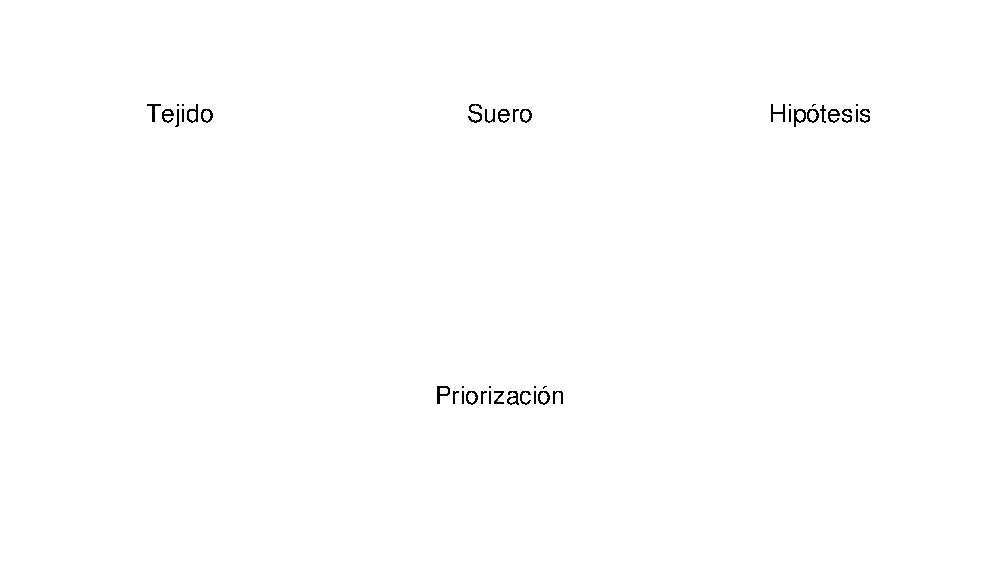
\includegraphics[width=0.92\textwidth]{figures/f01.pdf}
\caption{Cuatro bloques de la corrida: tejido, suero, hipótesis y priorización. El trazo une el orden de lectura. No representa una proteína que pasa del tumor a la sangre.}
\label{fig:mapa}
\end{figure}
\fuente{\texttt{scripts/v3/exportar\_sitio\_v3\_7.py}, figura \texttt{f01}, a partir de \texttt{results/v3\_7/}.}
\todojd{escribe tu interpretación de la figura \ref{fig:mapa}.}

\section{Tejido}
\begin{itemize}
\item Signo del tumor primario, Tanaka frente a CPTAC: \TejidoNum\ de \TejidoDen.
\item Metástasis hepática frente a mucosa: \TejidoMetaNum\ de \TejidoMetaDen.
\item Cobertura: \CoberturaNum\ de \CoberturaDen. Veredicto de H1: \HunoVeredicto.
\item Concordancia de NES: \GoConNum\ de \GoConDen.
\end{itemize}
\begin{figure}[ht]
\centering

\includegraphics[width=0.84\textwidth]{figures/f05.pdf}
\caption{Cada punto es un gen de la tabla de H7 medido también en Tanaka. El eje horizontal es el \(\log_2\)FC de CPTAC y el vertical, el de Tanaka.}
\label{fig:tejido}
\end{figure}
\fuente{\texttt{results/v3\_7/}, figura \texttt{f05}.}
\todojd{escribe tu interpretación de la figura \ref{fig:tejido}. No afirmes que el signo compartido localiza una muestra.}

\begin{figure}[ht]
\centering

\includegraphics[width=0.84\textwidth]{figures/f07.pdf}
\caption{Cada punto es un término con FDR de CPTAC dentro del umbral y con NES en Tanaka.}
\label{fig:go}
\end{figure}
\fuente{\texttt{results/v3\_7/go\_tejido.json}, figura \texttt{f07}.}
\todojd{escribe tu interpretación de la figura \ref{fig:go}. Un ORA de cero términos en Tanaka no es ausencia de biología: Tanaka tiene \GoTanakaSuben\ términos ORA que suben y \GoTanakaBajan\ que bajan, y \GoTanakaGsea\ con GSEA.}

\section{Suero}
\begin{table}[ht]
\caption{Celda preregistrada del suero, CP frente a CN}
\label{tab:celda}
\begin{tabular}{lr}
\toprule
Clase & Proteínas \\
\midrule
Diferentes & \SueroDif \\
Equivalentes & \SueroEq \\
Indeterminadas & \SueroInd \\
Total & \SueroN \\
\bottomrule
\end{tabular}
\end{table}
\fuente{\texttt{results/v3\_7/suero\_embudo.json}, campo \texttt{celda\_preregistrada}.}
\todojd{El cero no lleva un segmento inventado. No escribas que la equivalencia estadística es identidad biológica.}

\begin{figure}[ht]
\centering
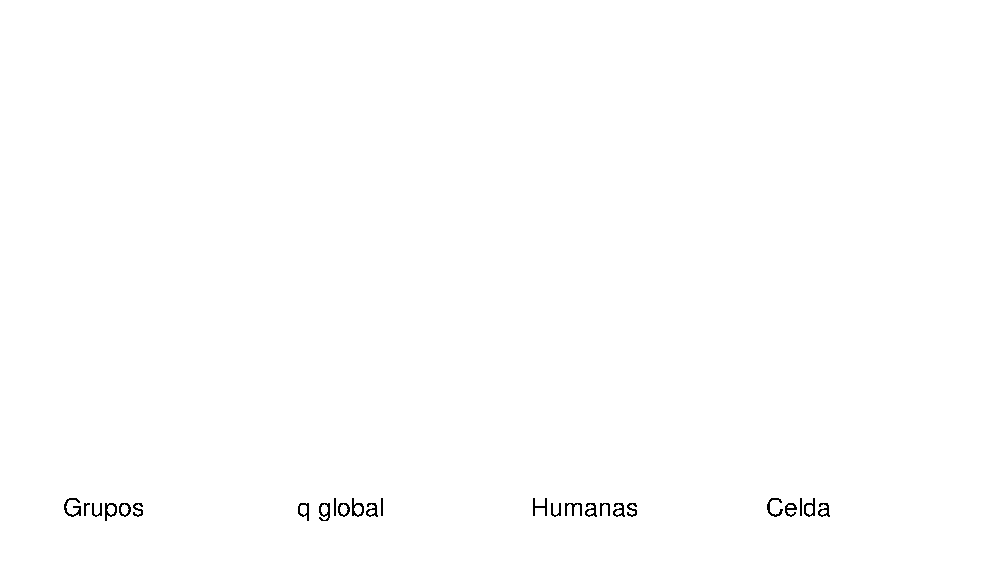
\includegraphics[width=0.92\textwidth]{figures/f02.pdf}
\caption{Embudo del suero. Alturas: \EmbudoGrupos\ grupos, \EmbudoQ\ con el filtro global, \EmbudoHumanos\ humanas y la celda de \SueroN.}
\label{fig:embudo}
\end{figure}
\fuente{\texttt{results/v3\_7/suero\_embudo.json}, figura \texttt{f02}.}
\todojd{escribe tu interpretación de la figura \ref{fig:embudo}.}

\begin{figure}[ht]
\centering
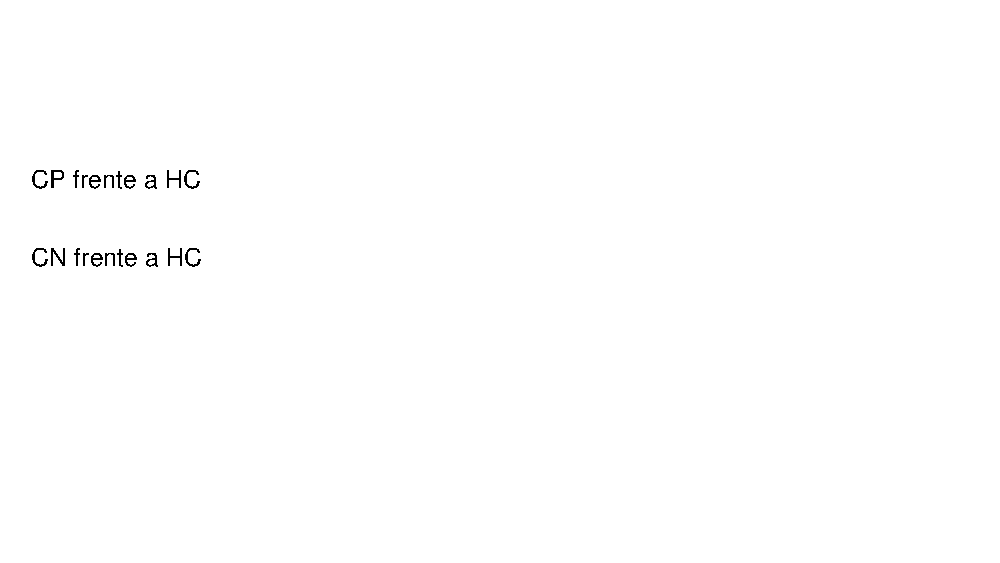
\includegraphics[width=0.84\textwidth]{figures/f03.pdf}
\caption{La barra superior es CP frente a CN. Las de abajo son los contrastes con HC, medido aparte: \HcCpDif\ diferentes en CP y \HcCnDif\ en CN. HC no decide la pregunta.}
\label{fig:hc}
\end{figure}
\fuente{\texttt{suero\_k4\_crc\_sanos.tsv} y \texttt{suero\_k4\_cn\_sanos.tsv}, figura \texttt{f03}.}
\todojd{escribe tu interpretación de la figura \ref{fig:hc}. No llames sanos a CN.}

\section{Calidad, orden y modelos}
\begin{itemize}
\item Preanalítica: estado \PreEstado. Crudos válidos: \PreCrudos. Con fecha: \PreFecha. AUC del orden: \PreAuc. p exacta de Mann-Whitney: \(1{,}5\times 10^{-11}\). Es el valor de \texttt{cifras.tex} (\texttt{\textbackslash PreP}); va en fórmula porque la fuente no tiene el signo de exponente.
\item M2, todas las proteínas: AUC \MlTodas. M3, solo calidad: \MlCalidad. M5, sin la calidad: \MlSinCalidad, p \MlSinCalidadP.
\item M1: \MlHumana. M4, coagulación: \MlCoagulacion. M6: \MlPca.
\end{itemize}
\begin{figure}[ht]
\centering
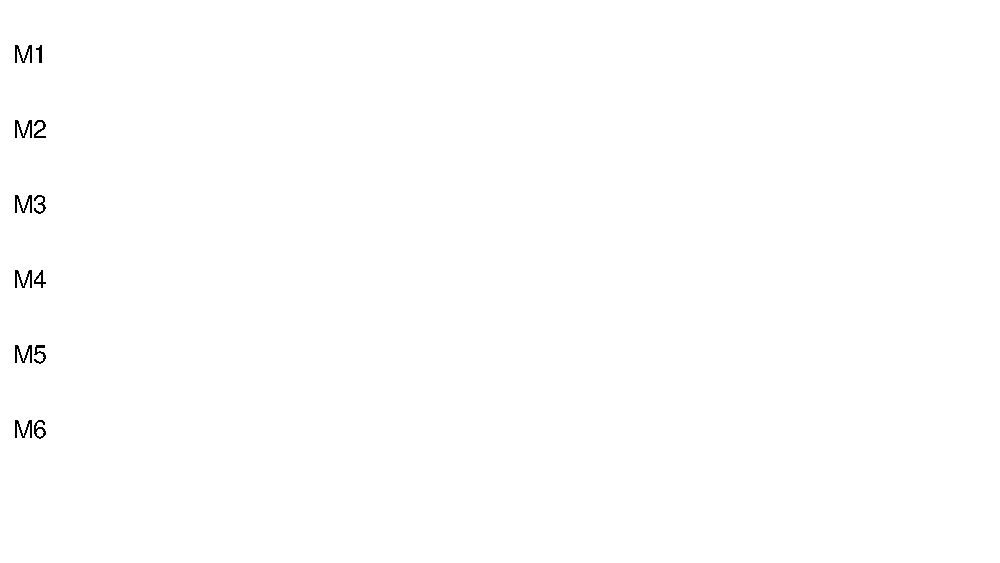
\includegraphics[width=0.84\textwidth]{figures/f08.pdf}
\caption{AUC fuera de pliegue de M1 a M6. La línea discontinua es el percentil 95 del nulo de K5.}
\label{fig:auc}
\end{figure}
\fuente{\texttt{results/v3\_7/ml\_suero\_permutacion.json}, figura \texttt{f08}.}
\todojd{escribe tu interpretación de la figura \ref{fig:auc}. No presentes el AUC como sensibilidad ni como especificidad de un examen.}

\begin{figure}[ht]
\centering
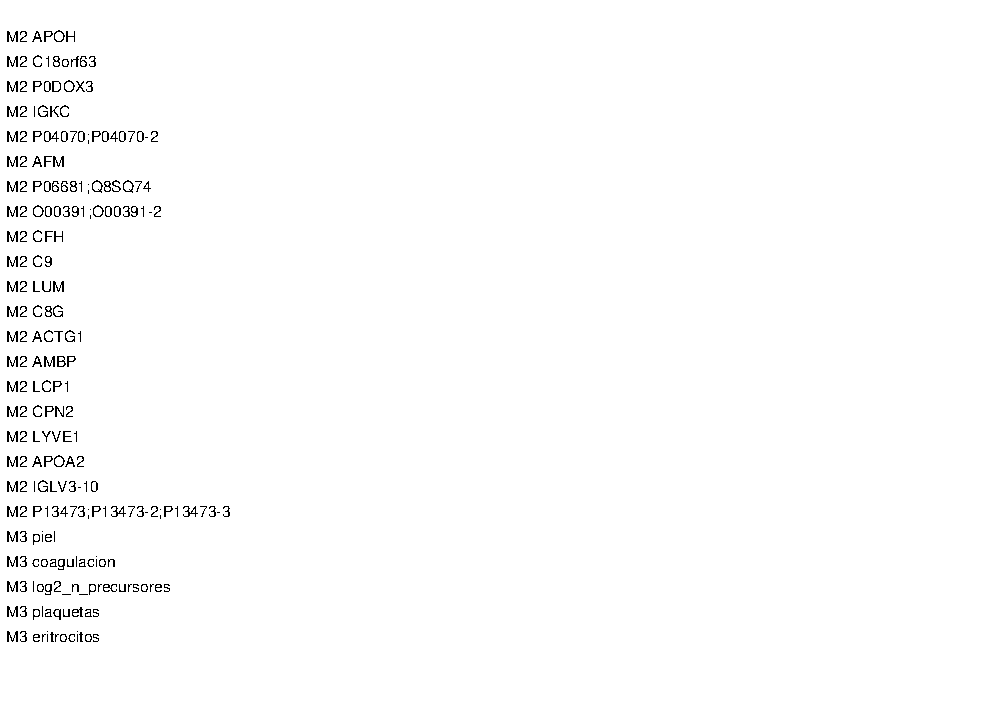
\includegraphics[width=0.78\textwidth]{figures/f09.pdf}
\caption{Media del valor absoluto de SHAP en M2 y en M3. M3 usa las variables de calidad que trae el fichero.}
\label{fig:shap}
\end{figure}
\fuente{Figura \texttt{f09}.}
\todojd{escribe tu interpretación de la figura \ref{fig:shap}.}

\section{Hipótesis y priorización}
\begin{table}[ht]
\caption{Estado de las hipótesis en la corrida firmada}
\label{tab:hipotesis}
\begin{tabular}{llp{7.2cm}}
\toprule
Hipótesis & Estado & Cifra que sí está \\
\midrule
H5 & \HcincoEstado & \HcincoUniverso\ genes en el universo principal. Fracción pan-carcinoma 0,119. Clasifica 624 proteínas. \\
H6 & \HseisEstado & No informa a favor ni en contra. \\
H7 & \HsieteEstado & Álvez 2023: AUC \HsieteAlvez. HPA: AUC \HsieteHpa. Secundario: \HsieteSec, con vector en \HsieteNEsm\ y \HsieteOmitidas\ omitidas. \\
H8 & \HochoEstado & \HochoTumorales\ tumorales epiteliales en \HochoUniverso. \\
H9 & \HnueveEstado & No decide la tesis. \\
H10 & \HdiezEstado & \HdiezN\ proteínas. \\
\bottomrule
\end{tabular}
\end{table}
\fuente{JSON \texttt{h5} a \texttt{h10} de \texttt{results/v3\_7/}.}
\todojd{El intervalo de Álvez es 0,381 a 0,584 (53 y 73) y el del HPA es 0,353 a 0,573 (53 y 63). Papier 2024 queda no evaluable: 1 y 125. Escribe eso solo si usas H7.}

\begin{itemize}
\item Pasos de priorización: \PrioriPasoUno, \PrioriPasoDos, \PrioriPasoTres, \PrioriPasoCuatro, \PrioriPasoCinco, \PrioriPasoSeis\ y \PrioriPasoSiete.
\item Del paso 5, \PrioriBajan\ bajan en CPTAC y \PrioriSuben\ suben.
\item Multiverso: \MultiSuero\ celdas de suero, \MultiMl\ de aprendizaje, \MultiDif\ con alguna proteína diferente.
\end{itemize}
\begin{figure}[ht]
\centering

\includegraphics[width=0.84\textwidth]{figures/f04.pdf}
\caption{Rejilla de \MultiSuero\ celdas. El trazo discontinuo marca las que tienen alguna proteína diferente. No es una cohorte nueva.}
\label{fig:multi}
\end{figure}
\fuente{\texttt{results/v3\_7/multiverso\_resumen.json}, figura \texttt{f04}.}
\todojd{escribe tu interpretación de la figura \ref{fig:multi}.}

\begin{figure}[ht]
\centering
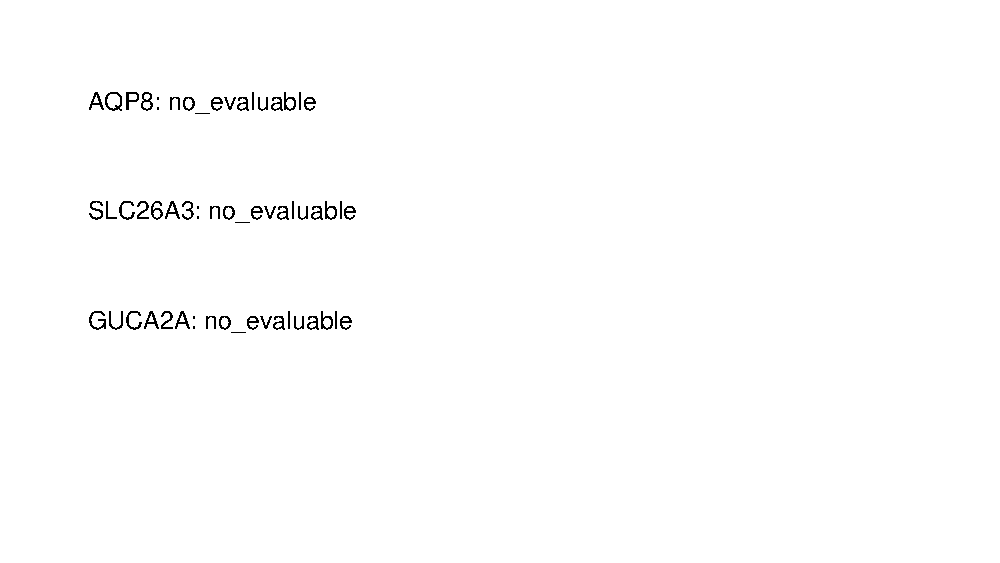
\includegraphics[width=0.7\textwidth]{figures/f06.pdf}
\caption{Controles de tejido no medibles. AQP8, GUCA2A y SLC26A3 quedan con trazo discontinuo porque el fichero no los da para la prueba.}
\label{fig:controles}
\end{figure}
\fuente{Figura \texttt{f06}. [PENDIENTE: verificar en \texttt{results/v3\_7/} el veredicto de CA1 antes de escribirlo en la prosa. El anexo viejo decía «CA1 pasa» y no se copió aquí.]}
\todojd{escribe tu interpretación de la figura \ref{fig:controles} solo con el fichero que abras.}
